\subsubsection{Định nghĩa}
Xử lý ngôn ngữ tự nhiên (Natural language processing - NLP) là một lĩnh vực phụ liên ngành của khoa học máy tính và tìm kiếm thông tin. Mục tiêu chính của nó là cung cấp cho máy tính khả năng hỗ trợ và thao tác với ngôn ngữ của con người. NLP liên quan đến việc xử lý các tập dữ liệu ngôn ngữ tự nhiên, chẳng hạn như kho văn bản hoặc kho dữ liệu giọng nói, bằng cách sử dụng các phương pháp học máy dựa trên quy tắc hoặc xác suất (tức là thống kê và gần đây nhất là dựa trên mạng nơ-ron). Mục tiêu là giúp máy tính có khả năng ``hiểu'' nội dung của các tài liệu, bao gồm cả sắc thái theo ngữ cảnh của ngôn ngữ trong đó. Vì mục đích này, xử lý ngôn ngữ tự nhiên thường vay mượn các ý tưởng từ ngôn học lý thuyết. Sau đó, công nghệ có thể trích xuất chính xác thông tin và hiểu biết có trong tài liệu, cũng như phân loại và tổ chức các tài liệu đó.

Những thách thức trong xử lý ngôn ngữ tự nhiên thường liên quan đến nhận dạng giọng nói, hiểu ngôn ngữ tự nhiên và tạo ngôn ngữ tự nhiên.

NLP có nguồn gốc từ những năm 1940 khi Alan Turing đã xuất bản một bài báo có tựa đề ``Computing Machinery and Intelligence'' đề xuất thứ hiện nay được gọi là Bài kiểm tra Turing làm tiêu chuẩn cho trí thông minh, mặc dù vào thời điểm đó nó không được coi là một vấn đề riêng biệt so với trí tuệ nhân tạo. Bài kiểm tra được đề xuất bao gồm một nhiệm vụ liên quan đến việc giải nghĩa và tạo ra ngôn ngữ tự nhiên một cách tự động. Sau đó quá trình phát triển của NLP gồm có 3 giai đoạn chính:
% https://en.wikipedia.org/wiki/Natural_language_processing
\begin{itemize}
    \item Symbolic NLP (1950 - đầu 1990): Tiền đề của NLP được trình bày bởi thí nghiệm Chinese Room của John Searle: Cung cấp cho máy tính một bộ quy tắc (ví dụ: sách hội thoại tiếng Trung, với các câu hỏi và câu trả lời tương ứng), máy tính mô phỏng khả năng hiểu ngôn ngữ tự nhiên (hoặc các tác vụ NLP khác) bằng cách áp dụng các quy tắc đó vào dữ liệu nó gặp phải.
    \item Statistical NLP (1990s-2010s): Cho đến những năm 1980, hầu hết các hệ thống xử lý ngôn ngữ tự nhiên đều dựa trên các bộ quy tắc phức tạp được viết bằng tay. Tuy nhiên, bắt đầu từ cuối những năm 1980, đã có một cuộc cách mạng trong lĩnh vực xử lý ngôn ngữ tự nhiên với việc đưa ra các thuật toán học máy cho xử lý ngôn ngữ. Điều này là do sự gia tăng ổn định về sức mạnh tính toán (định luật Moore) và sự giảm dần vai trò thống trị của các lý thuyết ngôn ngữ học theo Chomsky, những lý thuyết này không khuyến khích ngôn ngữ học dựa trên kho dữ liệu (corpus linguistics) - nền tảng của phương pháp học máy trong xử lý ngôn ngữ ngày nay.
    \item Neural NLP (hiện tại): Vào năm 2003, mô hình n-gram là thuật toán thống kê tốt nhất để xử lý ngôn ngữ tự nhiên. Tuy nhiên, Yoshua Bengio cùng các cộng sự đã vượt qua mô hình này bằng cách sử dụng mạng Perceptron đa lớp (có một lớp ẩn và khả năng xử lý ngữ cảnh của nhiều từ, được huấn luyện trên 14 triệu từ). Đến năm 2010, Tomáš Mikolov (khi đó là nghiên cứu sinh tiến sĩ tại Đại học Công nghệ Brno) cùng các cộng sự đã áp dụng mạng nơ-ron hồi quy đơn giản với một lớp ẩn vào xử lý ngôn ngữ. Sau đó, ông tiếp tục phát triển Word2vec. Và như thế, trong những năm tiếp theo của thập kỉ, việc học biểu diễn và các phương pháp học máy theo phong cách mạng nơ-ron sâu (có nhiều lớp ẩn) đã trở nên phổ biến trong lĩnh vực xử lý ngôn ngữ tự nhiên. 
\end{itemize}

\subsubsection{Các bước xử lý trong xử lý ngôn ngữ tự nhiên}

Phân tích hình thái: Đây là bước đầu tiên trong xử lý văn bản, nhằm nhận biết, phân tích và miêu tả cấu trúc của từng đơn vị ngôn ngữ, chẳng hạn như từ gốc, biên từ, phụ tố, từ loại, v.v. Các bài toán điển hình trong phần này là tách từ (word segmentation) và gán nhãn từ loại (part-of-speech tagging) trong xử lý tiếng Việt. 

Phân tích cú pháp: Phân tích cú pháp là quá trình phân tích một chuỗi các biểu tượng ngôn ngữ theo cú pháp của ngôn ngữ. Đầu vào là một câu văn và đầu ra là một cây phân tích thể hiện cấu trúc cú pháp của câu đó. Các phương pháp thường dùng trong phân tích cú pháp là văn phạm phi ngữ cảnh (context-free grammar - CFG), văn phạm danh mục kết nối (combinatory categorial grammar - CCG), và văn phạm phụ thuộc (dependency grammar - DG). 

Phân tích ngữ nghĩa: Phân tích ngữ nghĩa nhằm tìm ra ý nghĩa của các đơn vị ngôn ngữ và xác định mối quan hệ ngữ nghĩa giữa chúng, từ cấp độ từ vựng đến cấp độ cú pháp. Điều này liên quan đến việc hiểu được các từ và câu trong bối cảnh ngữ nghĩa của chúng.
 
Phân tích diễn ngôn: Phân tích diễn ngôn xem xét mối quan hệ giữa ngôn ngữ và ngữ cảnh sử dụng, thực hiện ở mức đoạn văn hoặc toàn bộ văn bản thay vì chỉ ở mức câu. Điều này giúp hiểu rõ hơn ý nghĩa và tầm quan trọng của một đoạn văn trong ngữ cảnh tổng thể của văn bản. 

\subsubsection{Một vài ứng dụng của xử lý ngôn ngữ tự nhiên}

Xử lý ngôn ngữ tự nhiên được ứng dụng rộng rãi trong nhiều khía cạnh của cuộc sống và công việc. Trong suốt hơn nửa thế kỷ, NLP đã phát triển đáng kể và đem lại nhiều ứng dụng đột phá. 

\begin{figure}[htb]
    \centering
    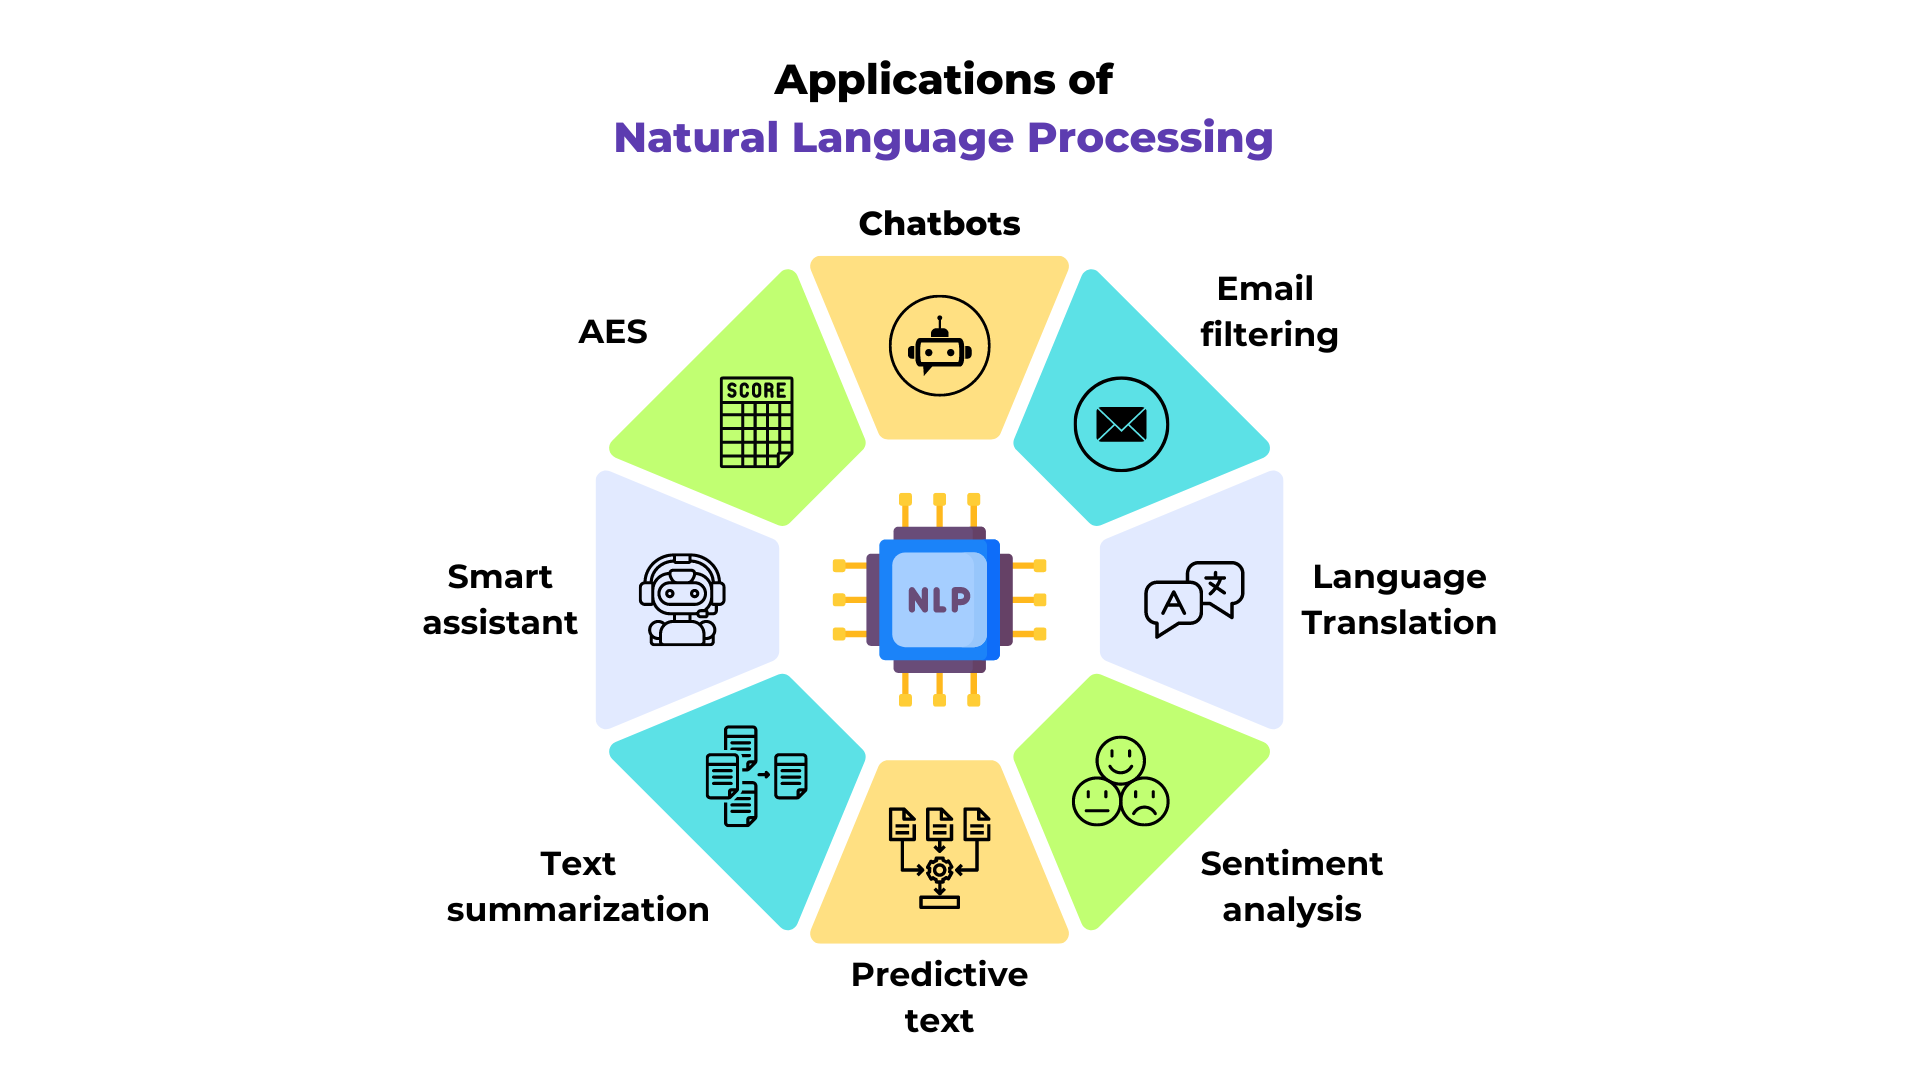
\includegraphics[width=\textwidth]{image/applications-of-nlp.png}
    \caption{Minh họa một số ứng dụng của xử lý ngôn ngữ tự nhiên}
    \label{fig:applications-of-nlp}
    % \source{https://www.analyticsvidhya.com/blog/2021/06/what-is-nlp-and-its-applications/}'
\end{figure}

\begin{itemize}
    \item Nhận dạng giọng nói (Automatic Speech Recognition - ASR, hoặc Speech To Text - STT) là một trong những ứng dụng tiêu biểu của xử lý ngôn ngữ tự nhiên. Với sự tiến bộ của các thuật toán và công nghệ, việc chuyển đổi từ tiếng nói sang văn bản đã trở nên chính xác hơn. Hệ thống nhận dạng giọng nói ngày càng phổ biến trong các ứng dụng hỗ trợ khách hàng, điều khiển thiết bị qua giọng nói và ghi chú cuộc họp.
    \item Tổng hợp giọng nói (Speech synthesis hoặc Text to Speech – TTS) là một ứng dụng ngược lại, cho phép máy tính đọc văn bản một cách tự nhiên và sinh động. Công nghệ tổng hợp giọng nói đang ngày càng tiến xa, giúp giọng nói của các chatbot và trợ lý ảo trở nên sống động và giống thực tế hơn, tạo sự tương tác tự nhiên và gần gũi hơn với con người.
    \item Trả lời câu hỏi (Question Answering - QA) là một bài toán phức tạp trong xử lý ngôn ngữ tự nhiên, yêu cầu máy tính hiểu và trả lời câu hỏi dưới dạng ngôn ngữ tự nhiên. Một hệ thống QA hiệu quả cần kết hợp các phương pháp như trích xuất thông tin, phân tích ngữ pháp và xử lý ngữ nghĩa. Đối với những câu hỏi đơn giản, hệ thống trả lời câu hỏi có thể đưa ra câu trả lời chính xác. Tuy nhiên, với những câu hỏi phức tạp hơn hoặc yêu cầu hiểu sâu hơn, các thách thức vẫn còn tồn tại và đòi hỏi sự phát triển thêm của xử lý ngôn ngữ tự nhiên. 
    \item Tóm tắt văn bản tự động (Automatic Text Summarization) là một ứng dụng quan trọng trong việc thu gọn và tóm tắt thông tin quan trọng từ văn bản gốc. Có hai phương pháp chính trong tóm tắt, là trích xuất và tóm lược ý. Trong trích xuất, hệ thống sẽ chọn các câu hoặc đoạn văn từ văn bản gốc, giữ lại những thông tin quan trọng nhất. Trong tóm lược ý, hệ thống sẽ tạo ra những câu tóm tắt mới dựa trên ngữ cảnh của văn bản. 
    \item Chatbot là một trong những ứng dụng phổ biến nhất của xử lý ngôn ngữ tự nhiên. Nhờ vào sự tiến bộ của các mô hình học máy và xử lý ngôn ngữ tự nhiên, chatbot ngày càng trở nên thông minh và có khả năng giao tiếp một cách tự nhiên. Chatbot được sử dụng trong nhiều lĩnh vực như hỗ trợ khách hàng, dự đoán thời tiết, đặt lịch hẹn và nhiều ứng dụng thú vị khác. 
    \item Dịch máy (Machine Translation - MT) là một trong những ứng dụng cổ điển nhất và đồng thời cũng là một trong những thách thức lớn trong xử lý ngôn ngữ tự nhiên. Với sự ra đời của mô hình dịch máy sử dụng mạng nơ-ron (neural machine translation), chất lượng dịch ngày càng được cải thiện và có thể đáp ứng nhu cầu của người dùng trong nhiều tình huống giao tiếp quốc tế. 
    \item Tạo hình ảnh từ văn bản (Text-to-image generation): Mô hình này có khả năng nhận dạng mô tả bằng ngôn ngữ tự nhiên và tạo ra hình ảnh tương ứng với mô tả đó. Sự phát triển của các ứng dụng này bắt đầu vào giữa những năm 2010, cùng với sự bùng nổ của Trí tuệ Nhân tạo (AI) nhờ những tiến bộ trong lĩnh vực mạng nơ-ron sâu. Đến năm 2022, chất lượng đầu ra của các mô hình tiên tiến như DALL-E 2 của OpenAI, Imagen của Google Brain, Stable Diffusion của Stability AI và Midjourney đã được đánh giá là gần tương đương với ảnh chụp thực tế và tranh vẽ của con người.
    \item Phân tích cảm xúc: Phân tích cảm xúc được sử dụng để xác định và phân loại ý định cảm xúc ẩn chứa trong văn bản. Kỹ thuật này bao gồm việc phân tích văn bản để xác định xem cảm xúc được thể hiện là tích cực, tiêu cực hay trung lập. Các mô hình phân loại cảm xúc thường sử dụng các đầu vào như chuỗi n-gram của từ, đặc trưng do con người tạo hoặc sử dụng các mô hình học sâu được thiết kế để nhận dạng cả các phụ thuộc dài hạn và ngắn hạn trong chuỗi văn bản. Ứng dụng của phân tích cảm xúc rất đa dạng, mở rộng sang các nhiệm vụ như phân loại đánh giá của khách hàng trên các nền tảng trực tuyến khác nhau.
\end{itemize}